\chapter*{Обзор литературы}

% \section{Параметры производительности для управления распространением пучка}
% Несмотря на разнообразие способов управления распространением пучка, все они должны подчиняться нескольким физическим принципам, чтобы соответствовать параметрам производительности, необходимым для реальных приложений. А именно, пучок должен быть достаточно узким и подчиняться управлению в большом диапазоне углов, называемом полем зрения (FOV, field of view): вплоть до 180$^\circ$ для одномерного сканирования и до полусферы для двухмерного сканирования. Кроме того, угол излучения должен перенастраиваться в реальном времени на высокой скорости с минимальными потерями интенсивности. 

% Диаграмма направленности (ДН) $F (\vec \xi\,)$ устройства управления пучком может быть определена из его ближнего электромагнитного поля $E(\vec r\,)$ с помощью преобразования Фурье:
% \begin{equation}
%     \label{1}
%     F(\vec \xi\,) = \iint E(\vec r\,)\, e^{ik_0\left(\vec r \cdot \vec \xi\,\right)}\, d^2\vec r,
% \end{equation}
% где вектор $\vec \xi = (\phi, \Theta)$ показывает полярное и азимутальное направления, \mbox{$\vec r = (x, y)$} указывает на точку на фазированной антенной решетке (ФАР). $k_0$ --- волновое число. Положим ближнее поле $u(\vec r\,)$ каждой антенны одинаковым. Тогда суммарное ближнее поле можно записать как
% \begin{equation}
%     \label{2}
%     E(\vec r\,) = \sum_n C_n\, u(\vec r - \vec r_n) = u(\vec r\,)* \sum_n C_n \, \delta(\vec r - \vec r_n),
% \end{equation}
% где комплексные коэффициенты $C_n$ описывают описывают фазы и амплитуды излучателей, а символ $*$ обозначает свертку. $\delta(\vec r\,)$ --- двумерная дельта-функция. В соответствии с теорией антенн, диаграмма направленности ФАР является произведением ДН отдельных элементов и ДН $U(\xi\,)$ идентичной решетки с изотропными антеннами:
% \begin{equation}
%     F(\vec \xi\,) = U(\vec \xi\,)\,\sum_n C_n\, e^{ik_0\,\vec r_n \cdot \vec \xi}.
% \end{equation}

\section{Обобщенный закон Снелла}

Пусть каждой точке $M(x)$ границы раздела соответствует значение фазы, равное $\Phi(x)$ и пусть падающая на границу раздела волна, проходящая через заданную точку $M(x)$, претерпевает фазовый разрыв $\Phi(x)$. Для такой границы мы вынуждены пересмотреть классический закон Снелла, описываемый формулой
\begin{equation}
    n_i \sin \Theta_i = n_t \sin \Theta_t
\end{equation}
в соответствии с принципом Ферма.

Рассмотрим плоскую волну, падающую под углом $\Theta_i$ . Если предположить, что два пути бесконечно близки к реальному пути света (Рис. \ref{fig:generalized}А), то разность фаз между ними равна нулю
\begin{equation}
    \label{eq:opticalPathLengthDifference}
    [k_0n_i\sin\Theta_i\, dx + (\Phi + d\Phi)] - [k_0n_t\sin\Theta_t\,dx + \Phi] = 0,
\end{equation}
где $\Theta_t$ --- угол преломления; $\Phi$ и $\Phi + d\Phi$ --- разрывы фаз в местах пересечения границы раздела синим и красным путями соответственно; $dx$ --- расстояние между точками пересечения; $n_i$ и $n_t$ --- показатели преломления двух сред; $k_0 = 2\pi/\lambda_0$ --- волновое число, где $\lambda_0$ --- длина волны в вакууме. Если градиент фазы $d\Phi/dx$ создан постоянным, предыдущее уравнение \eqref{eq:opticalPathLengthDifference} приводит к обобщенному закону преломления Снелла
\begin{equation}
    \label{eq:generalizedRefraction}
    n_t\sin\Theta_t - n_i \sin\Theta_i = \frac{\lambda_0}{2\pi}\frac{d\Phi}{dx}.
\end{equation}

Уравнение \eqref{eq:generalizedRefraction} показывает, что преломленный луч может иметь произвольное направление при условии, что создан подходящий постоянный градиент фазы $d\Phi/dx$ вдоль границы раздела (Рис.~\ref{fig:generalized}Б) \cite{generalized2011}. Более того, при ненулевом градиенте фазы два угла падения $\pm \Theta_i$ соответствуют различным углам преломления. Как следствие, существуют два угла полного внутреннего отражения
\begin{equation}
    \Theta_c = \arcsin \left(\pm\frac{n_t}{n_i} - \frac{\lambda_0}{2\pi}\frac{d\Phi}{dx}\right)
\end{equation}

Аналогично, для отражения имеем
\begin{equation}
    \label{eq:generalizedReflection}
    \sin\Theta_r - \sin\Theta_i = \frac{\lambda_0}{2\pi n_i}\frac{d\Phi}{dx},
\end{equation}
где $\Theta_r$ --- угол отражения. Между $\Theta_r$ и $\Theta_i$ существует нелинейная связь, которая заметно отличается от известного закона геометрической оптики. Уравнение \eqref{eq:generalizedReflection} показывает, что всегда существует критический угол падения
\begin{equation}
    \Theta_c' = \arcsin\left(1 - \frac{\lambda_0}{2\pi n_i}\left|\frac{d\Phi}{dx}\right|\right),
\end{equation}
при котором отраженная волна становится эванесцентной.

Такая возможность управления распространением пучка привела к созданию структур, реализующих различные градиенты фазы --- метаповерхностей.

\begin{figure}
    \begin{center}
        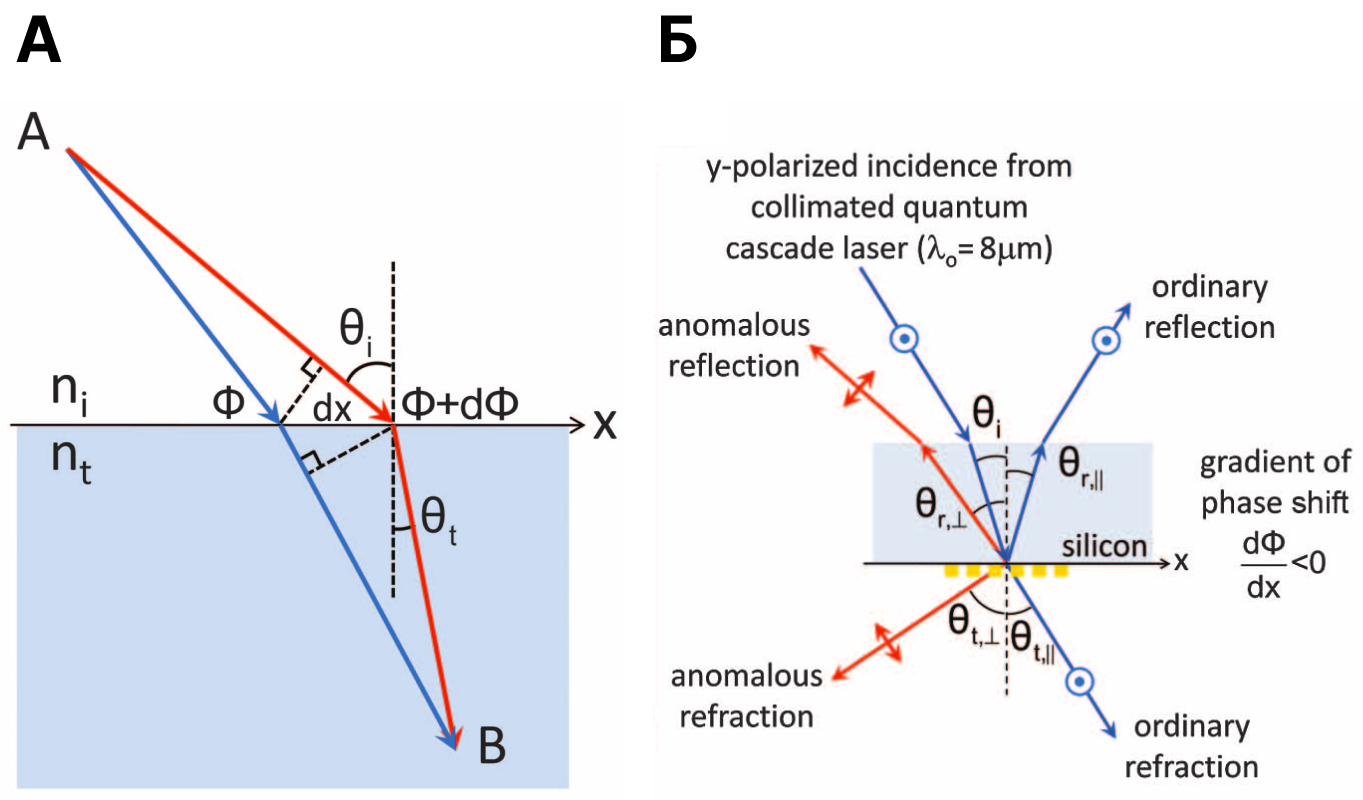
\includegraphics[width=0.92\textwidth]{pictures/Generalized_Snell's_law.png}
        \caption{\textbf{(А)} Рисунок, используемый для вывода обобщенного закона преломления Снелла. Граница между двумя средами искусственно структурирована так, чтобы внести резкий фазовый сдвиг на пути света, который зависит от положения на границе раздела. $\Phi$ и $\Phi + d\Phi$ — фазовые сдвиги, при которых два луча (синий и красный) пересекают границу.\cite[Fig. 1]{generalized2011} \textbf{(Б)} Схема экспериментальной установки, демонстрирующей обобщенный закон Снелла.\cite[Fig. 3B]{generalized2011}}
    \end{center}
    \label{fig:generalized}
\end{figure}

\section{Метаповерхности}

Метаповерхности градиента активной фазы (метаповерхности) представляют собой структуры субволновых оптических элементов --- антенн, реализующих пространственно изменяющийся фазовый разрыв (т. е. градиент фазы) для падающей плоской волны. Фаза взаимодействующего света определяется геометрией антенн и характеристиками материала изготовления метаповерхности и может иметь вид, например, такой, как на Рис. \ref{fig:metasurfaces}Б. Пример такой метаповерхности из V-образных антенн приведен на Рис. \ref{fig:metasurfaces}А. За счёт наличия градиента фазы, в соответствии с обобщенным законом Снелла, наблюдается как нормальный прошедший пучок, так и аномальный, отклоняющийся на угол, определяемый \eqref{eq:generalizedRefraction}. Для активного управления распространением пучка метаповерхности используются совместно с методом когерентного контроля.

\begin{figure}
    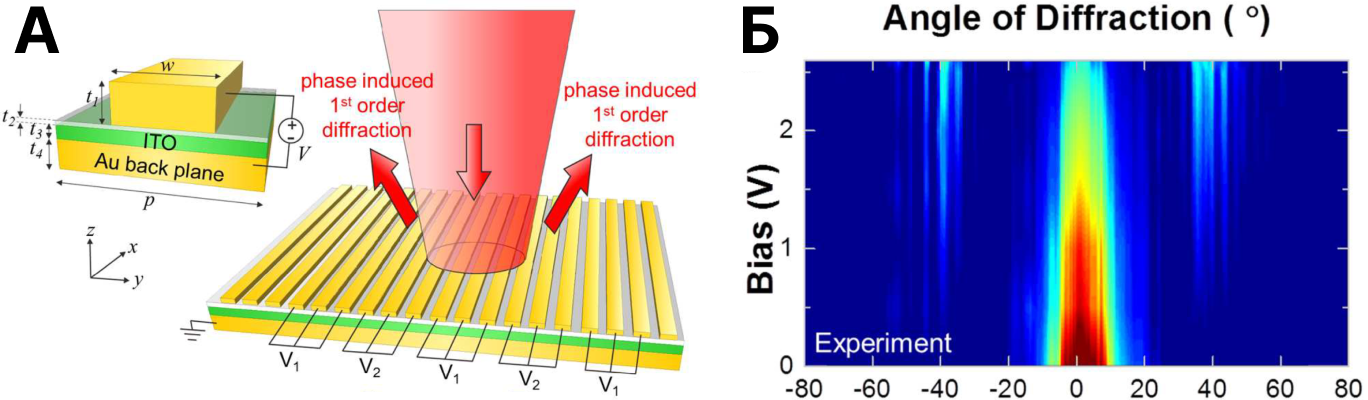
\includegraphics[width=\textwidth]{pictures/Metasurfaces.png}
    \caption{\textbf{(А)} Рисунок, показывающий наличие и направление распространения нормального и аномального прошедших пучков и их поляризацию. Крупным планом изображены детали конструкции V-образной антенны. \cite[Fig. 1A]{coherentControl2014} \textbf{(Б)} Зависимость фазового разрыва от координаты точки падения пучка для структуры из V-образных антенн.\cite[Fig. 1D]{coherentControl2014}}
    \label{fig:metasurfaces}
\end{figure}

\section{Когерентный контроль}

Метод когерентного контроля в общем случае заключается в изучении зависимости интерференционной картины, полученной после взаимодействия двух когерентных пучков, распространяющихся в противоположных направлениях, с оптически неоднородной средой (структурой), от разности фаз этих пучков. При таком взаимодействии в пространстве образуется стоячая электромагнитная волна, и степень влияния неоднородности на интерференционную картину определяется положениями пучностей и узлов относительно структуры. При рассмотрении сред, линейные размеры которых по направлению распространения излучения (толщина) значительно меньше длины волны, можно выделить два предельных случая:
\begin{enumerate}
    \item Структура находится в узле стоячей волны. Тогда неоднородность становится <<выключенной>> и практически не влияет на распространение излучения.
    \item Структура находится в пучности. Тогда влияние неоднородности максимально.
\end{enumerate}
За счёт этих двух состояний можно реализовывать полностью оптическое переключение, а рассмотрев другие предельные случаи, даже реализовать базовые логические операции (Рис. \ref{fig:opticalLogic})\cite{twoDimensional2016}.
\begin{figure}
    \begin{center}
        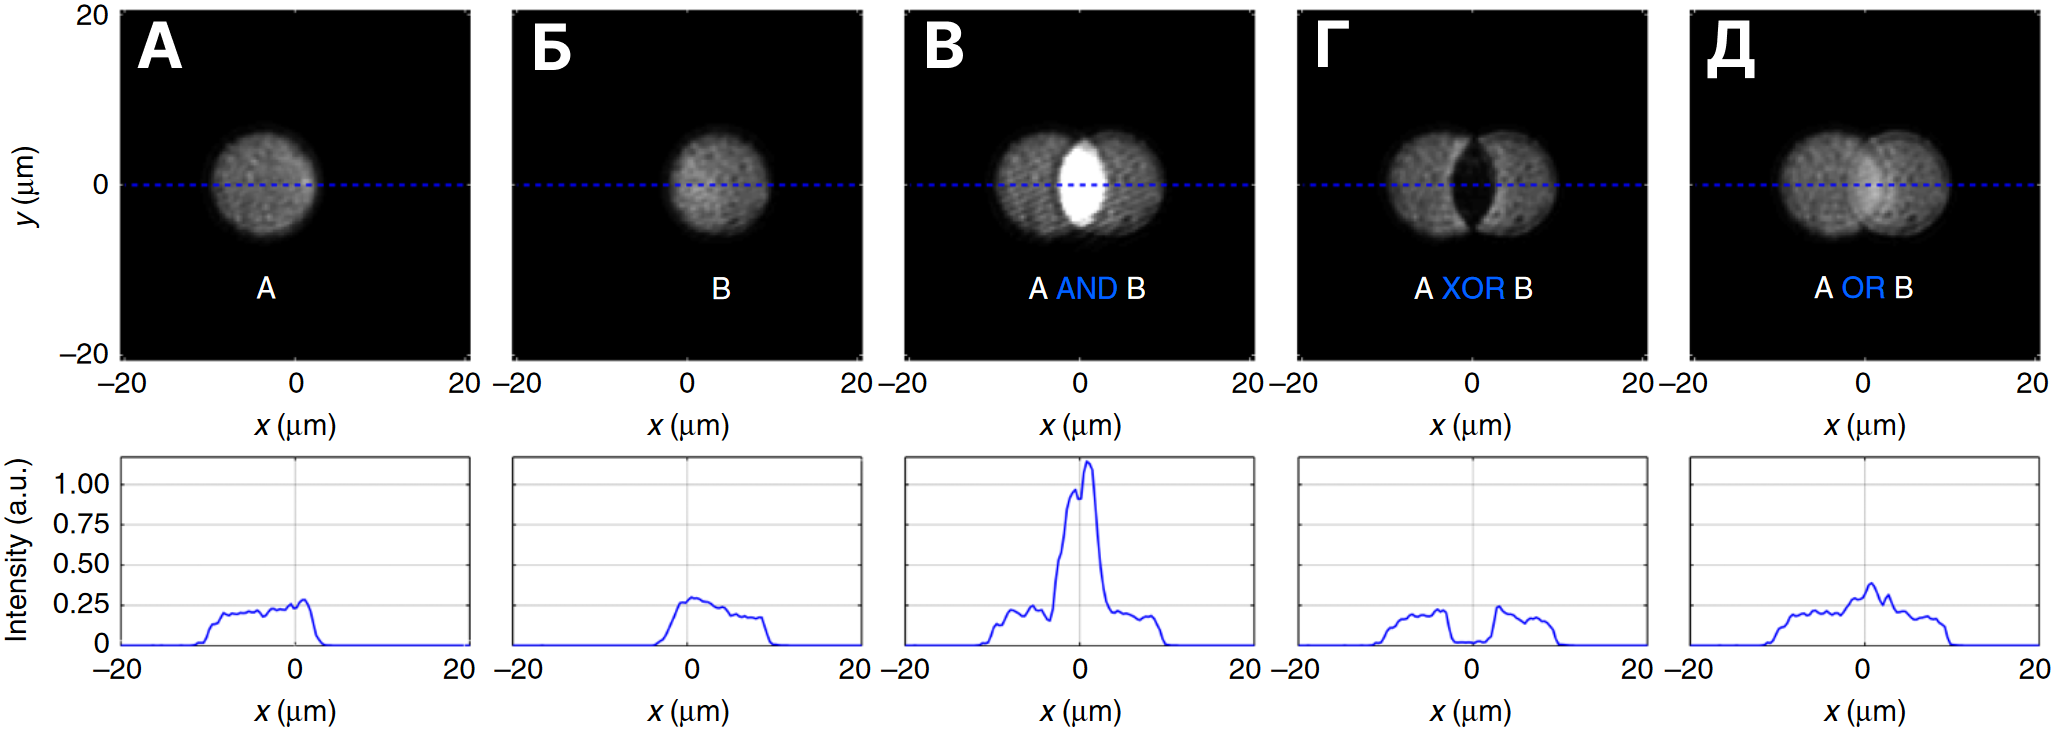
\includegraphics[width=\textwidth]{pictures/Optical_logic.png}
        \caption{Оптические базовые логические операции. Изображения метаповерхности, \textbf{(А)} освещенной только лучом $A$, \textbf{(Б)} только лучом $B$ и \textbf{(В-Д)} обоими лучами $A$ и $B$. Разным относительным фазам лучей $A$ и $B$ соответствуют разные логические операции: \textbf{(В)} $A$ И $B$ ($\Theta = \pi$), \textbf{(Г)} $A$ <<ИСКЛЮЧАЮЩЕЕ ИЛИ>> $B$ ($\Theta = 0$) и \textbf{(Д)} $A$ ИЛИ $B$ ($\Theta = \pm \pi/3$). На графиках показан профиль интенсивности вдоль соответствующей пунктирной синей линии. Уровни интенсивности показаны в одинаковых оттенках серого на всех изображениях и в одном вертикальном масштабе на всех графиках.\cite[Fig. 3]{twoDimensional2016}}
    \end{center}
    \label{fig:opticalLogic}
\end{figure}

